% Beamer slide template prepared by Tom Clark <tom.clark@op.ac.nz>
% Otago Polytechnic
% Dec 2012

\documentclass[10pt]{beamer}
\usetheme{Dunedin}
\usepackage{graphicx}
\usepackage{fancyvrb}
\newcommand\codeHighlight[1]{\textcolor[rgb]{1,0,0}{\textbf{#1}}}

\title{Working With Relational Databases: SQLAlchemy}
\author[IN710]{OOSD}
\institute[Otago Polytechnic]{
  School of Information Technology \\
  Otago Polytechnic \\
  Dunedin, New Zealand \\
}
\date{}
\begin{document}

%----------- titlepage ----------------------------------------------%
\begin{frame}[plain]
  \titlepage
\end{frame}

\begin{frame}
	\frametitle{A very common problem}
	\begin{itemize}
		\item We want to work with persistent data.
		\item A relational database is a very common place to keep such data.
		\item Moving data between an object oriented model and a relational database is tricky.
		\item Also, we want to avoid DBMS-specific code in our applications.
	\end{itemize}
\end{frame}

\begin{frame}
	\frametitle{A very common solution}
	\begin{itemize}
		\item There are many libraries for working with databases in every language.
		\item Some are very nice, some are less so.  Most of them work ok.
		\item A common pattern they implement it \emph{Object-Relational Mapping} (ORM).
		\item There is, however, a degree of pushback against ORM.
	\end{itemize}
\end{frame}

\begin{frame}
	\frametitle{SQLAlchemy}
	\begin{itemize}
		\item SQLAlchemy is an excellent set of libraries for working with databases in Python.
		\item It supports ORM, but does not require it.
		\item It's very flexible.  Many DB libraries sacrifice flexibility in return for simplicity.
	\end{itemize}
\end{frame}

\begin{frame}
	\frametitle{SQLAlchemy Components}
	
	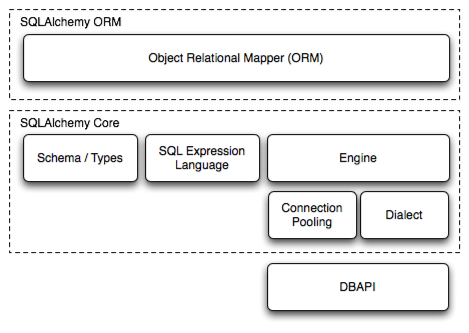
\includegraphics[scale=0.6]{sqla_arch_small.png}
	
\end{frame}
\begin{frame}
	\frametitle{ORM}
	\begin{itemize}
		\item The ORM in SQLAlchemy moves data back-and-forth between application code and a database.
		\item It converts types between those supported by the DBMS and Python types.
	\end{itemize}
\end{frame}
\begin{frame}
	\frametitle{SQLAlchemy Example}
	
	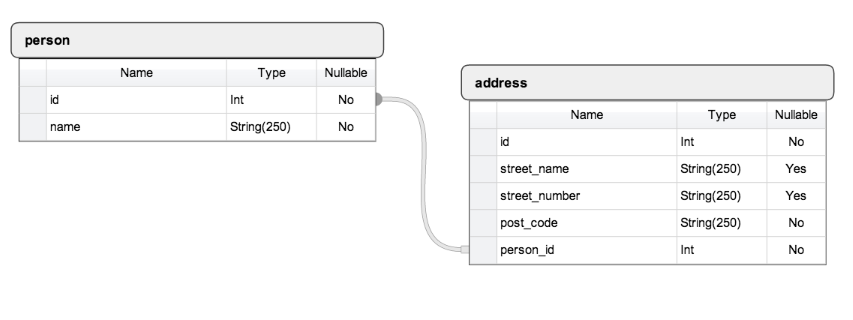
\includegraphics[scale=0.4]{erd.png}
	
\end{frame}

\begin{frame}[fragile]
	\frametitle{Person class}
	\begin{verbatim}
	Base = declarative_base()
	
    class Person(Base):
        __tablename__ = 'person'
        id = Column(Integer, primary_key=True)
        name = Column(String(250), nullable=False)
	\end{verbatim}
\end{frame}

\begin{frame}[fragile]
	\frametitle{Address class}
	\begin{verbatim}
    class Address(Base):
        __tablename__ = 'address'
        id = Column(Integer, primary_key=True)
        street_name = Column(String(250))
        street_number = Column(String(250))
        post_code = Column(String(250), nullable=False)
        person_id = Column(Integer, ForeignKey('person.id'))
        person = relationship(Person)
	
	\end{verbatim}
\end{frame}

\begin{frame}[fragile]
	\frametitle{Creating the database}
	\begin{verbatim}
    engine = create_engine('sqlite:///sqlalchemy_example.db')
    Base.metadata.create_all(engine)
	\end{verbatim}
\end{frame}

\begin{frame}[fragile]
	\frametitle{Getting a Record }
	\begin{verbatim}
	# ... some boilerplate above
	session.query(Person).all()
	session.query(Person).get(id)
	session.query(Person).filter(Person.name == name)
	\end{verbatim}
\end{frame}

\begin{frame}[fragile]
	\frametitle{Updating a Record }
	\begin{verbatim}
	session = DBSession()
	# get a Person
	# modify a Person
	session.add(person)
	session.commit()
	\end{verbatim}

\end{frame}
\begin{frame}
	\frametitle{References}
	
	\begin{itemize}
		\item SQLAlchemy Documentation:
		\url{http://docs.sqlalchemy.org/en/rel_1_0/index.html}
		\item Handy tutorial:
		\url{http://www.pythoncentral.io/introductory-tutorial-python-sqlalchemy/}
		\item Installing SQLALchemy: 
		\url{http://www.pythoncentral.io/how-to-install-sqlalchemy/}
	\end{itemize}
\end{frame}

\begin{frame}
	\frametitle{Exercise}
	\begin{itemize}
		\item Write a set of classes using SQLAlchemy that
		model students, semesters, and papers.  Use SQLite for persistence.
		\item Write a script that lets me 
		\begin{itemize}
			\item List students
			\item List papers
			\item Select a paper and see some details for the paper plus a list of students.
			\item Select a student and a semester and print the students schedule for the semester.
		\end{itemize}
	\end{itemize}
\end{frame}


\end{document}
